%
% compile with pdflatex:
%   $ pdflatex homework-hw
% , yields homework-example.pdf
%    You might need to compile twice, if, e.g., you start using references
%

\documentclass[10pt,letterpaper,oneside]{article}
\usepackage[ascii]{inputenc}
\usepackage{graphicx}
\graphicspath{ {} }
\usepackage{amsmath,amsfonts,amssymb}
\usepackage[margin=1in]{geometry}
	\setlength{\parindent}{0em}
	\setlength{\parskip}{1em}



\newtheorem{theorem}{Theorem}

%%%% user definitions %%%%%%%%%%%%%%%%%%%%%%%

\newcommand{\Problem}[1]{\subsection*{Problem #1}}
\newcommand{\Part}[1]{\subsubsection*{Part #1}}
\newcommand{\Solution}{\subsubsection*{Solution}}

	% Forms for Big-Oh notation
\DeclareMathOperator{\Omicron}{O}
\DeclareMathOperator{\omicron}{o}

\newcommand{\BigOh}[1]{\Omicron(#1)}
\newcommand{\LittleOh}[1]{\omicron(#1)}
\newcommand{\BigOmega}[1]{\Omega(#1)}
\newcommand{\LittleOmega}[1]{\omega(#1)}
\newcommand{\BigTheta}[1]{\Theta(#1)}

	% Operators for dominance notation
\newcommand{\domeq}{\sim}
\newcommand{\domle}{\preceq}
\newcommand{\domlt}{\prec}
\newcommand{\domge}{\succeq}
\newcommand{\domgt}{\succ}

\newcommand\tab[1][1cm]{\hspace*{#1}}


%%%%%%%%  You edit stuff below this line  %%%%%%%%%%%%%%%%%%%%%%%%%%

\title{HW8 Theory}
\author{Alexander Kazantsev}
%\date{}  % uses today, by default

\begin{document}
\maketitle
\Problem{6.6}
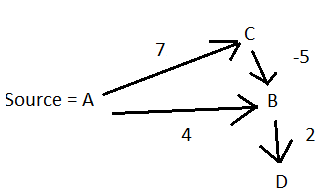
\includegraphics{graph.png}

First $A$ is popped out of the queue and  and edges $(A,C)$ and $(A,B)$ are relaxed. B is popped off and relax the edge $(B,D)$ giving a distance of 6. $D$ is now at the top, but has no edges. $C$ is the last vertex left. The edge $(C, B)$ is relaxed giving a total distance to $B$ as 2. Now the queue is empty, but the shortest path to $B$ from $A$ is not correct.

\Problem{7.1}
Insert( val, v, adjList)

	\tab assert v $\in$ adjList

	\tab if val !$\in$ adjList

	\tab\tab add(adjList, val)

	\tab\tab ListInsert(adjList[ v ], val)

	\tab else

	\tab\tab ListInsert(adjList[ v ], val)
\\
\\
\\
\\
\\
\\
Delete(val, vertex,adjList)

	\tab assert val and vertex $\in$ adjList

	\tab $\forall$ $e$ $\in$ adjList [ val ]

	\tab\tab if e == vertex

	\tab\tab\tab remove(adjList[ vertex ], e)

	\tab\tab\tab break

	\tab $\forall$ $e$ $\in$ adjList [ vertex ]

	\tab\tab if e == val

	\tab\tab\tab remove(adjList[ val ], e)

	\tab\tab\tab break
\Problem{7.2}
Restructuring the adjacency list as a matrix would allow for removal of the first edge in constant time. The down side is that this derivative requires more space than a linked list implementation. 

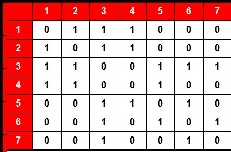
\includegraphics{AdjacencyMatrix.jpg}

DeleteFirstEdge(vertex, adjMatrix)

	\tab assert vertex $\in$ adjList

	\tab adjMatrix[ vertex[ 0 ] ] [ vertex ] = Null

	\tab adjMatrix[ vertex ] [ 0 ] = Null

\Problem{7.3}
\Part{a}
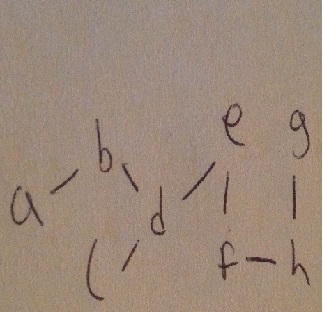
\includegraphics{a.jpg}
\Part{b}
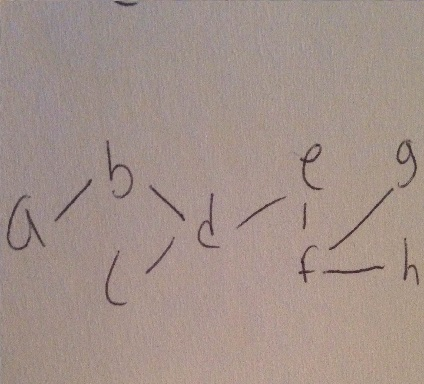
\includegraphics{b.jpg}
\maketitle
\end{document}